%%%%%% -*- Coding: utf-8-unix; Mode: latex

\documentclass[polish]{projectreport}

\usepackage[utf8]{inputenc}
\usepackage{url}
\usepackage{subfigure}
\usepackage{tabularx}
\usepackage{ragged2e}
\usepackage{booktabs}
\usepackage{multirow}
\usepackage{grffile}
\usepackage{float}

\usepackage[bookmarks=false]{hyperref}
\hypersetup{colorlinks,
  linkcolor=blue,
  citecolor=blue,
  urlcolor=blue}

\usepackage{indentfirst}
\usepackage{caption}
\usepackage{listings}
\usepackage[ruled,linesnumbered,lined]{algorithm2e}
\usepackage[svgnames]{xcolor}
\usepackage{inconsolata}
\usepackage{fancyhdr}

\usepackage{csquotes}
\DeclareQuoteStyle[quotes]{polish}
  {\quotedblbase}
  {\textquotedblright}
  [0.05em]
  {\quotesinglbase}
  {\fixligatures\textquoteright}
\DeclareQuoteAlias[quotes]{polish}{polish}

\usepackage[
style=numeric,
sorting=none,
isbn=false,
doi=true,
url=true,
backref=false,
backrefstyle=none,
maxnames=10,
giveninits=true,
abbreviate=true,
defernumbers=false,
backend=biber]{biblatex}
\addbibresource{bibliography.bib}

\lstset{
    basicstyle=\ttfamily\footnotesize,
    backgroundcolor=\color{gray!5},
    commentstyle=\it\color{Green},
    keywordstyle=\color{Red},
    stringstyle=\color{Blue},
    numberstyle=\tiny\color{Black},
    escapeinside=`',
    frame=single,
    tabsize=2,
    rulecolor=\color{black!30},
    title=\lstname,
    breaklines=true,
    breakatwhitespace=true,
    framextopmargin=2pt,
    framexbottommargin=2pt,
    extendedchars=false,
    captionpos=b,
    abovecaptionskip=5pt,
    keepspaces=true,
    numbers=left,
    numbersep=5pt,
    showspaces=false,
    showstringspaces=false,
    showtabs=false,
    tabsize=2
}

\SetAlgorithmName{\LangAlgorithm}{\LangAlgorithmRef}{\LangListOfAlgorithms}
\renewcommand{\lstlistingname}{\LangListing}
\renewcommand\lstlistlistingname{\LangListOfListings}

\newcolumntype{Y}{>{\small\centering\arraybackslash}X}
\captionsetup[figure]{skip=5pt,position=bottom}
\captionsetup[table]{skip=5pt,position=top}

%%%%%%%%%%%%%%%%%%%%%%%%%%%%%%%%%%%%%%%%%%%%%%%%%%%%%%%%%%%%%%%%%%%%%%%%%%%%%%%
\author{Wojciech Niemiec}

\title{Symulacja rozprzestrzeniania się chorób w populacji
z wykorzystaniem modelu agentowego}

\date{
    {\small Akademia Górniczo-Hutnicza im. Stanisława Staszica w Krakowie \\
    Wydział Informatyki \\
    \texttt{wnagh@student.agh.edu.pl}\\[2ex]%
    \the\year}
}

\pagestyle{fancy}
\fancyhf{}
\fancyhead[LE,RO]{\thepage}

%%%%%%%%%%%%%%%%%%%%%%%%%%%%%%%%%%%%%%%%%%%%%%%%%%%%%%%%%%%%%%%%%%%%%%%%%%%%%%%
\begin{document}

\maketitle
\thispagestyle{empty}

\begin{abstract}
\noindent W pracy przedstawiono agentowy model symulacji
rozprzestrzeniania się chorób zakaźnych, oparty na rozszerzeniu
klasycznego modelu SIR. Model uwzględnia sześć stanów agentów:
podatny (S -- susceptible), zarażony (I -- infected), odporny
(R -- recovered), zmarły (D -- dead), zaszczepiony (V -- vaccinated)
oraz poddany kwarantannie (Q -- quarantined). Parametry dobrano
na podstawie danych dotyczących pandemii COVID-19, przyjmując
Nową Zelandię jako punkt odniesienia dla parametrów interwencji. Przeprowadzono cztery eksperymenty badające wpływ
współczynnika zaraźliwości, strategii interwencji, tempa kampanii
szczepień oraz struktury wiekowej populacji na przebieg epidemii.
Symulacje wykonano w języku Python z użyciem biblioteki Mesa.

\noindent\textbf{Słowa kluczowe:} model agentowy, symulacja epidemii,
SIR, COVID-19, Mesa, Python
\end{abstract}

%%%%%%%%%%%%%%%%%%%%%%%%%%%%%%%%%%%%%%%%%%%%%%%%%%%%%%%%%%%%%%%%%%%%%%%%%%%%%%%
\section{\SectionTitleIntroduction}
\label{sec:introduction}

Modelowanie epidemii chorób zakaźnych jest jednym z podstawowych
narzędzi epidemiologii. Klasyczne modele kompartmentowe, takie jak
model SIR zaproponowany przez Kermacka i McKendricka~\cite{kermack1927contribution},
opisują przebieg epidemii za pomocą układów równań różniczkowych,
dzieląc populację na grupy według stanu zdrowotnego. Podejście to,
choć poprawne matematycznie, traktuje populację jako jednorodną
całość i nie uwzględnia indywidualnych mechanizmów interwencji,
takich jak izolacja pojedynczych osób czy selektywne szczepienia.

Modele agentowe pozwalają symulować zachowania poszczególnych
jednostek i ich lokalne interakcje~\cite{railsback2011agent}.
Każdy agent reprezentuje konkretną osobę, ma przypisany stan
zdrowotny oraz indywidualne cechy wpływające na przebieg choroby.
Takie podejście umożliwia uwzględnienie różnorodności populacji
i losowości kontaktów społecznych, co jest trudne do osiągnięcia
w modelach klasycznych.

Podczas pandemii COVID-19 modele symulacyjne okazały się istotnym
narzędziem wspierającym decyzje zdrowotne. Raport Imperial College
London~\cite{ferguson2020report} pokazał, że pozwalają oceniać
skuteczność różnych strategii interwencji jeszcze przed ich
wdrożeniem. Jako punkt odniesienia dla parametrów interwencji
wybrano Nową Zelandię -- kraj, który łącząc obowiązkową kwarantannę
z intensywną kampanią szczepień osiągnął poziom wyszczepienia
sięgający 90\% uprawnionych do końca 2021 roku~\cite{baker2022newzealand}.

Celem pracy jest implementacja rozszerzonego modelu agentowego
epidemii i analiza wpływu wybranych parametrów epidemiologicznych
oraz strategii interwencji na przebieg symulacji. Model
zaimplementowano w Pythonie z użyciem biblioteki
Mesa~\cite{kazil2020mesa}.

Raport zorganizowany jest następująco. Sekcja~\ref{sec:solution}
opisuje strukturę modelu i przyjęte założenia.
Sekcja~\ref{sec:experiments} przedstawia wyniki czterech
eksperymentów. Sekcja~\ref{sec:conclusions} zawiera wnioski
i kierunki dalszych badań.

%%%%%%%%%%%%%%%%%%%%%%%%%%%%%%%%%%%%%%%%%%%%%%%%%%%%%%%%%%%%%%%%%%%%%%%%%%%%%%%
\section{Opis modelu agentowego}
\label{sec:solution}

\subsection{Opis modelu i logika agenta}
\label{sec:model}

Do wykonania eksperymentów użyto modelowania opartego na agentach
(ABM -- Agent-Based Model), które rozszerza standardowe modele
epidemiologiczne o możliwość przypisania każdej jednostce
indywidualnych cech i zachowań. Użyty model wyróżnia sześć stanów
agenta:

\begin{itemize}
    \item podatny (S -- susceptible),
    \item zarażony (I -- infected),
    \item odporny (R -- recovered),
    \item zmarły (D -- dead),
    \item zaszczepiony (V -- vaccinated),
    \item poddany kwarantannie (Q -- quarantined).
\end{itemize}

Klasyczny model SIR został rozszerzony o trzy dodatkowe stany.
Każdy agent posiada trzy atrybuty: stan zdrowotny, grupę wiekową
(młody, dorosły, senior) oraz licznik dni pozostałych do końca
kwarantanny (domyślnie zero). Przyjęto uproszczony rozkład grup
wiekowych 20/60/20 jako przybliżenie struktury typowej populacji.

Grupa wiekowa wpływa na dwa parametry: tempo zdrowienia $\gamma$
oraz prawdopodobieństwo śmierci $\delta$. Dla grupy młodych parametry
te są mnożone odpowiednio przez 2.0 i 0.1, natomiast dla seniorów
przez 0.6 i 3.0. Wartości dla grupy dorosłych pozostają bez zmian.
Przyjęto założenie, że seniorzy mają istotnie wyższe ryzyko zgonu
w wyniku choroby, co jest zgodne z danymi epidemiologicznymi
dotyczącymi COVID-19 -- Levin et al.~\cite{levin2020age} wykazali,
że współczynnik IFR rośnie wykładniczo z wiekiem, osiągając wartość
ponad 4\% dla osób po 75. roku życia wobec poniżej 0.01\%
dla młodych dorosłych. Wolniejsze zdrowienie seniorów wynika
z gorszej ogólnej kondycji układu odpornościowego.

W badanym modelu agent to obiekt systemu posiadający unikalne ID,
atrybut opisujący grupę wiekową oraz stan zdrowotny. Agenci
rozmieszczeni są na siatce o rozmiarach $40 \times 40$ pól
w eksperymentach właściwych.
Wiele agentów może jednocześnie zajmować to samo pole.

W każdej turze symulacji agent wykonuje akcje zależne od swojego
aktualnego stanu. Agent w stanie D (zmarły) nie wykonuje żadnych
akcji. Agent w stanie Q (kwarantanna) nie porusza się ani nie zaraża
sąsiadów -- odczekuje przypisaną liczbę dni, po czym wraca do stanu
I i może ponownie wyzdrowieć lub umrzeć. Pozostałe stany wykonują
następujące akcje:

\begin{itemize}
    \item \textbf{Ruch} -- agent przemieszcza się na losowo wybrane
    sąsiadujące pole spośród ośmiu możliwych kierunków, zgodnie
    z sąsiedztwem Moore'a.

    \item \textbf{Zarażanie sąsiadów} -- chory agent podejmuje próbę
    zarażenia agentów na sąsiadujących polach. Podatny agent (S)
    zostaje zarażony z prawdopodobieństwem $\beta$. Zaszczepiony
    agent (V) może zostać zarażony z prawdopodobieństwem
    $\beta \cdot (1 - \varepsilon)$, gdzie $\varepsilon$ oznacza
    skuteczność szczepionki -- przyjęto założenie, że szczepionka
    zmniejsza ryzyko zarażenia, lecz nie eliminuje go całkowicie.

    \item \textbf{Zdrowienie lub zgon} -- na podstawie rozkładu
    losowego oraz parametrów $\delta$ i $\gamma$ (skorygowanych
    o grupę wiekową) stan chorego agenta może zmienić się na R
    (odporny) lub D (zmarły). Parametr $\delta$ jest sprawdzany
    jako pierwszy -- jeśli agent umiera, parametr $\gamma$ nie
    jest już sprawdzany.

    \item \textbf{Kwarantanna} -- z prawdopodobieństwem $q$ zarażony
    agent zostaje skierowany na kwarantannę, zmieniając stan na Q.
    Przez czas trwania kwarantanny agent pozostaje nieruchomy
    i nie zaraża sąsiadów.
\end{itemize}





%%%%%%%%%%%%%%%%%%%%%%%%%%%%%%%%%%%%%%%%%%%%%%%%%%%%%%%%%%%%%%%%%%%%%%%%%%%%%%%
\subsection{Parametry modelu}
\label{sec:parameters}

Parametry modelu oparto na kilku niezależnych publikacjach naukowych.
Ich wartości przedstawia Tabela~\ref{tab:parameters}, a uzasadnienie
znajduje się poniżej.

\begin{table}[H]
\centering
\caption{Parametry bazowe modelu}
\begin{tabularx}{\columnwidth}{@{}llY@{}} \toprule
\textbf{Parametr} & \textbf{Symbol} & \textbf{Wartość} \\ \midrule
Współczynnik zaraźliwości  & $\beta$    & 0.08 \\
Tempo zdrowienia           & $\gamma$   & 0.07 \\
Współczynnik śmiertelności & $\delta$   & 0.001 \\
Skuteczność szczepionki    & $\varepsilon$ & 0.84 \\
Tempo szczepień            & $\nu$      & 0.00 \\
Czas kwarantanny           & $q$        & 10 \\
Prawdop. kwarantanny       & $\rho$     & 0.00 \\
Liczba agentów             & $N$        & 1000 \\
Rozmiar siatki             & ---        & $40 \times 40$ \\
\bottomrule
\end{tabularx}
\label{tab:parameters}
\end{table}

Współczynnik zaraźliwości $\beta$, tempo zdrowienia $\gamma$ oraz
współczynnik śmiertelności $\delta$ dobrano na podstawie estymacji
modelu SIRD dla danych epidemiologicznych Zjednoczonego Królestwa
z okresu kwiecień 2020 -- wrzesień 2021~\cite{alencar2022uk}.
Autorzy wyestymowali parametry modelu metodą state-space z wykorzystaniem
filtra Kalmana, kalibrując model na rzeczywistych danych o przypadkach
i zgonach.

Skuteczność szczepionki $\varepsilon = 0.84$ przyjęto na podstawie
badania CDC obejmującego dorosłych hospitalizowanych z powodu
COVID-19 w Stanach Zjednoczonych -- skuteczność szczepionek
Pfizer-BioNTech i Moderna wyniosła 84\% w okresie 13--24 tygodni
po przyjęciu drugiej dawki~\cite{taubenberger2021mmwr}.

Czas kwarantanny $q = 10$ dni uzasadniają badania empiryczne
przeprowadzone na czterech kohortach uniwersyteckich -- Liu
et al.~\cite{liu2022quarantine} wykazali, że kwarantanna oparta
na testach PCR powinna wynosić właśnie 10 dni, aby utrzymać
ryzyko transmisji po jej zakończeniu poniżej 5\%.

Parametry $\nu$ i $\rho$ dotyczące szczepień i kwarantanny
przyjęto domyślnie jako zero, ponieważ stanowią zmienne
eksperymentalne badane w rozdziale~\ref{sec:experiments}.
Liczba agentów $N = 1000$ oraz rozmiar siatki $40 \times 40$
to parametry techniczne przyjęte jako uproszczenie obliczeniowe.


%%%%%%%%%%%%%%%%%%%%%%%%%%%%%%%%%%%%%%%%%%%%%%%%%%%%%%%%%%%%%%%%%%%%%%%%%%%%%%%
\subsection{Implementacja}
\label{sec:implementation}

Projekt zaimplementowano w języku Python 3.13 z wykorzystaniem
biblioteki Mesa~\cite{kazil2020mesa} w wersji 2.3.0. Do analizy
i wizualizacji wyników eksperymentów użyto bibliotek pandas, numpy
oraz matplotlib. Interaktywna wizualizacja oparta jest na bibliotece
mesa-viz-tornado. Projekt składa się z następujących plików:

\begin{lstlisting}
disease_simulation/
|-- simulation/
|   |-- agent.py         # agent logic
|   |-- model.py         # model and grid
|   `-- visualization.py # visualization server
|-- experiments/
|   `-- experiments.py   # batch experiments
|-- figures/             # output charts
`-- report/              # LaTeX report
\end{lstlisting}

Interaktywna wizualizacja umożliwia przeprowadzenie symulacji
z dowolnie wybranymi parametrami oraz obserwację wyników
w czasie rzeczywistym w przeglądarce internetowej. Panel boczny
zawiera suwaki pozwalające na modyfikację wszystkich parametrów
modelu bez konieczności ingerencji w kod źródłowy. Przykładowy
widok wizualizacji przedstawia Rysunek~\ref{fig:visualization}.

\begin{figure}[H]
  \centering
  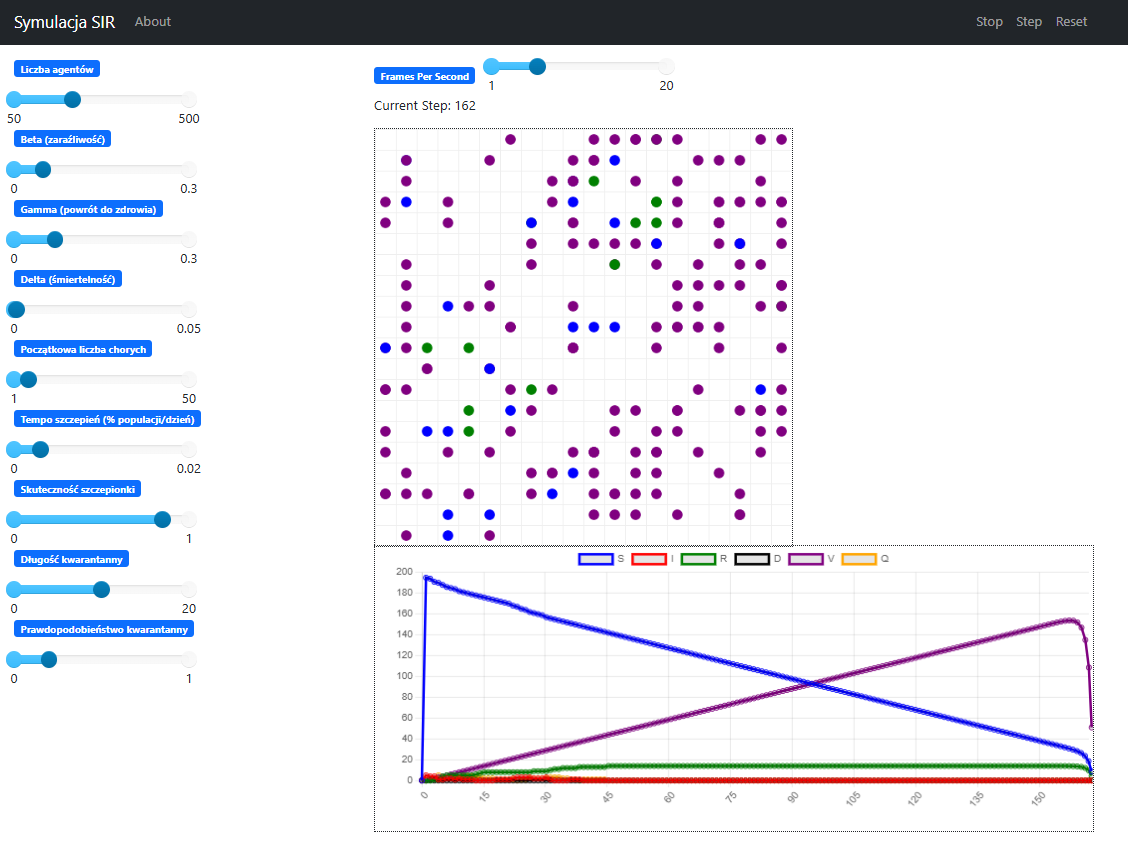
\includegraphics[width=0.8\textwidth]{figures/wizualizacja.png}
  \caption{Widok interaktywnej wizualizacji symulacji. Po lewej
  stronie panel z suwakami parametrów, po prawej siatka agentów
  (niebieski -- podatny, czerwony -- zarażony, zielony -- odporny,
  czarny -- zmarły, fioletowy -- zaszczepiony, pomarańczowy --
  kwarantanna) oraz wykres stanów SIRDVQ w czasie rzeczywistym.}
  \label{fig:visualization}
\end{figure}

Eksperymenty uruchamiane są z pliku \texttt{experiments.py}
i obejmują cztery pętle oparte na bazowych parametrach oraz na zmienianych wartościach poszczególnych zmiennych w celu zbadania różnych scenariuszy epidemii. Zakres obejmuje 300 dni od pierwszego zakażenia. Aby utrzymać stabilność wyników, każdą pętlę wykonano 30 razy i wyciągnięto średnią i odchylenie standardowe.

%%%%%%%%%%%%%%%%%%%%%%%%%%%%%%%%%%%%%%%%%%%%%%%%%%%%%%%%%%%%%%%%%%%%%%%%%%%%%%%
\section{\SectionTitleExperiments}
\label{sec:experiments}

\subsection{Eksperyment 1 -- Wpływ współczynnika zaraźliwości}
\label{sec:exp1}

Eksperyment bada wpływ współczynnika zaraźliwości $\beta$ na rozwój
i przebieg epidemii przy wyłączonych interwencjach, zgodnie z zasadą
ceteris paribus. Pozostałe parametry przyjmują wartości bazowe
z Tabeli~\ref{tab:parameters}.

\begin{figure}[H]
  \centering
  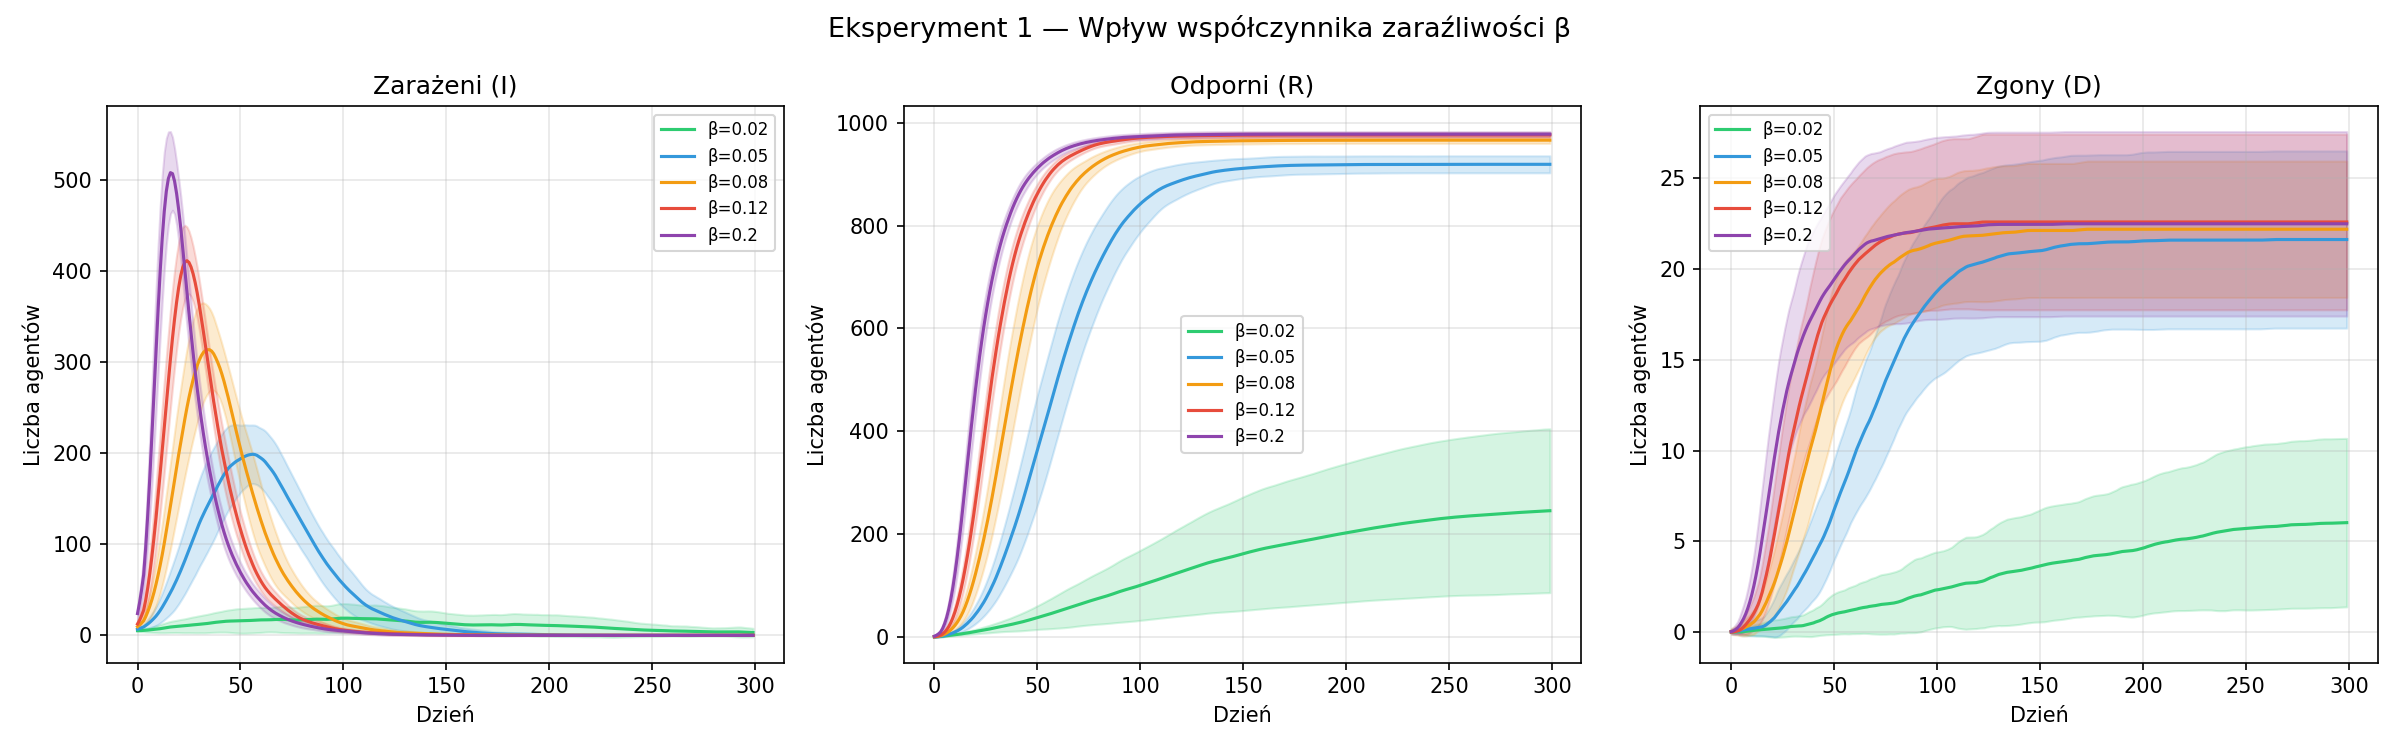
\includegraphics[width=\textwidth]{figures/exp1_beta.png}
  \caption{Wpływ współczynnika zaraźliwości $\beta$ na przebieg epidemii.
  Kolory odpowiadają wartościom $\beta \in \{0.02, 0.05, 0.08, 0.12, 0.20\}$.
  Zacieniowane obszary reprezentują odchylenie standardowe z 30 uruchomień.}
  \label{fig:exp1}
\end{figure}

Pierwszy wykres pokazuje liczbę zarażonych przy różnych wartościach
$\beta$. Wynik jest zgodny z oczekiwaniami -- im wyższa zaraźliwość,
tym szybciej osiągany jest szczyt zachorowań i tym krócej trwa
epidemia. Przypadek $\beta = 0.02$ jest szczególny -- choroba nie
osiągnęła wystarczającej zaraźliwości, aby rozprzestrzenić się
w całej populacji, co skutkowało minimalną liczbą zachorowań
i samoistnym wygaszeniem epidemii.

Drugi wykres przedstawia nabywanie odporności przy założeniu braku
kampanii szczepień. Dla wartości $\beta \geq 0.05$ już około 50.
dnia znacząca większość populacji nabywa odporność naturalną.
Ponownie wyróżnia się przypadek $\beta = 0.02$ -- widoczne jest
tu znacznie większe odchylenie standardowe względem pozostałych
wariantów, co wynika z wysokiej losowości przy tak niskim
współczynniku zaraźliwości.

Trzeci wykres przedstawia łączną liczbę zgonów. W porównaniu
do poprzednich wykresów odchylenie standardowe jest wysokie
we wszystkich wariantach -- jest to efekt małego prawdopodobieństwa
zgonu $\delta$, przy którym losowość ma duży wpływ na wynik.
Interesującą obserwacją jest zbliżona śmiertelność dla
$\beta \geq 0.08$, pomimo różnic w szczycie zachorowań.
Wynika to z tzw. efektu wyczerpania populacji podatnej
(\textit{burnout effect}) -- przy bardzo wysokiej zaraźliwości
epidemia przebiega tak gwałtownie, że chorzy zdrowieją lub
umierają zanim zdążą zarazić kolejne osoby, co paradoksalnie
ogranicza łączną liczbę zgonów względem wariantów o umiarkowanej
zaraźliwości.

%%%%%%%%%%%%%%%%%%%%%%%%%%%%%%%%%%%%%%%%%%%%%%%%%%%%%%%%%%%%%%%%%%%%%%%%%%%%%%%
\subsection{Eksperyment 2 -- Porównanie strategii interwencji}
\label{sec:exp2}

Eksperyment porównuje cztery scenariusze interwencji: brak działań,
sama kwarantanna, same szczepienia oraz połączenie obu metod.
Parametry interwencji oparto na danych z Nowej Zelandii~\cite{baker2022newzealand}
-- tempo szczepień wynosi 0.3\%/dzień, prawdopodobieństwo kwarantanny
$\rho = 0.3$, czas izolacji $q = 10$ dni.

\begin{figure}[H]
  \centering
  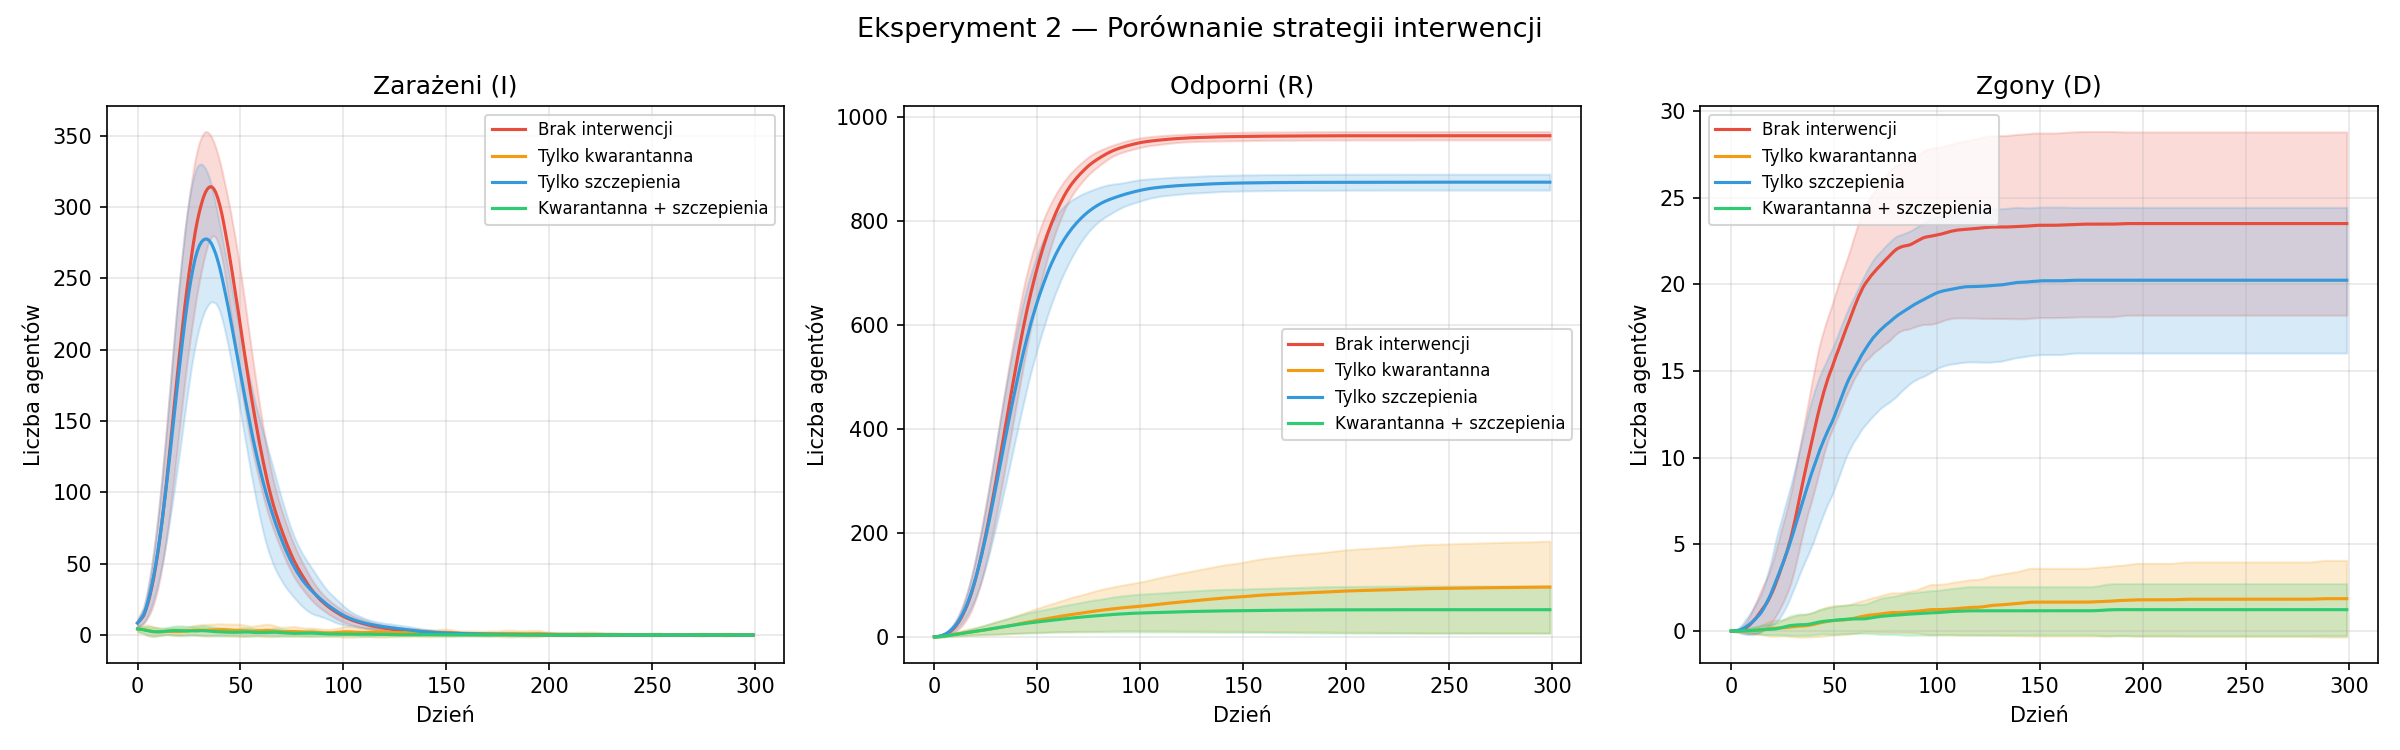
\includegraphics[width=\textwidth]{figures/exp2_interventions.png}
  \caption{Porównanie strategii interwencji: brak interwencji, sama
  kwarantanna, same szczepienia oraz połączenie obu metod.
  Zacieniowane obszary reprezentują odchylenie standardowe z 30 uruchomień.}
  \label{fig:exp2}
\end{figure}

Pierwszy wykres pokazuje wyraźne różnice w liczbie zarażonych między
scenariuszami. Brak interwencji i same szczepienia dają podobny
szczyt zachorowań -- szczepienia przy tempie 0.3\%/dzień nie
nadążają za rozprzestrzenianiem się epidemii we wczesnej fazie.
Kwarantanna natomiast niemal całkowicie eliminuje zachorowania,
co wynika z założeń modelowych -- agent objęty kwarantanną jest
w pełni izolowany i nie zaraża sąsiadów. W rzeczywistości skuteczność
izolacji jest niższa ze względu na nieprzestrzeganie zasad i kontakty
domowe, co stanowi ograniczenie modelu.

Drugi wykres pokazuje nabytą odporność. Scenariusz bez interwencji
i ze szczepieniami osiągają wysoką odporność populacyjną przez
naturalne przechorowanie -- odpowiednio około 950 i 850 agentów.
Przy samej kwarantannie liczba odpornych jest bardzo niska, co
oznacza że epidemia jest kontrolowana, ale populacja pozostaje
podatna -- potencjalnie narażona na kolejną falę po zniesieniu
restrykcji.

Trzeci wykres potwierdza że połączenie kwarantanny i szczepień
niemal eliminuje zgony. Sama kwarantanna redukuje je znacząco,
natomiast same szczepienia przy przyjętym tempie kampanii dają
efekt zbliżony do braku interwencji -- co sugeruje, że przy
$\beta = 0.08$ tempo 0.3\%/dzień jest niewystarczające do
skutecznej ochrony populacji bez wsparcia izolacji.

\subsection{Eksperyment 3 -- Wpływ tempa kampanii szczepień}
\label{sec:exp3}

Eksperyment bada jak tempo szczepień wpływa na przebieg epidemii.
Wartość 0.3\%/dzień odpowiada średniemu tempu kampanii w Nowej
Zelandii~\cite{baker2022newzealand}, pozostałe wartości stanowią
scenariusze porównawcze.

\begin{figure}[H]
  \centering
  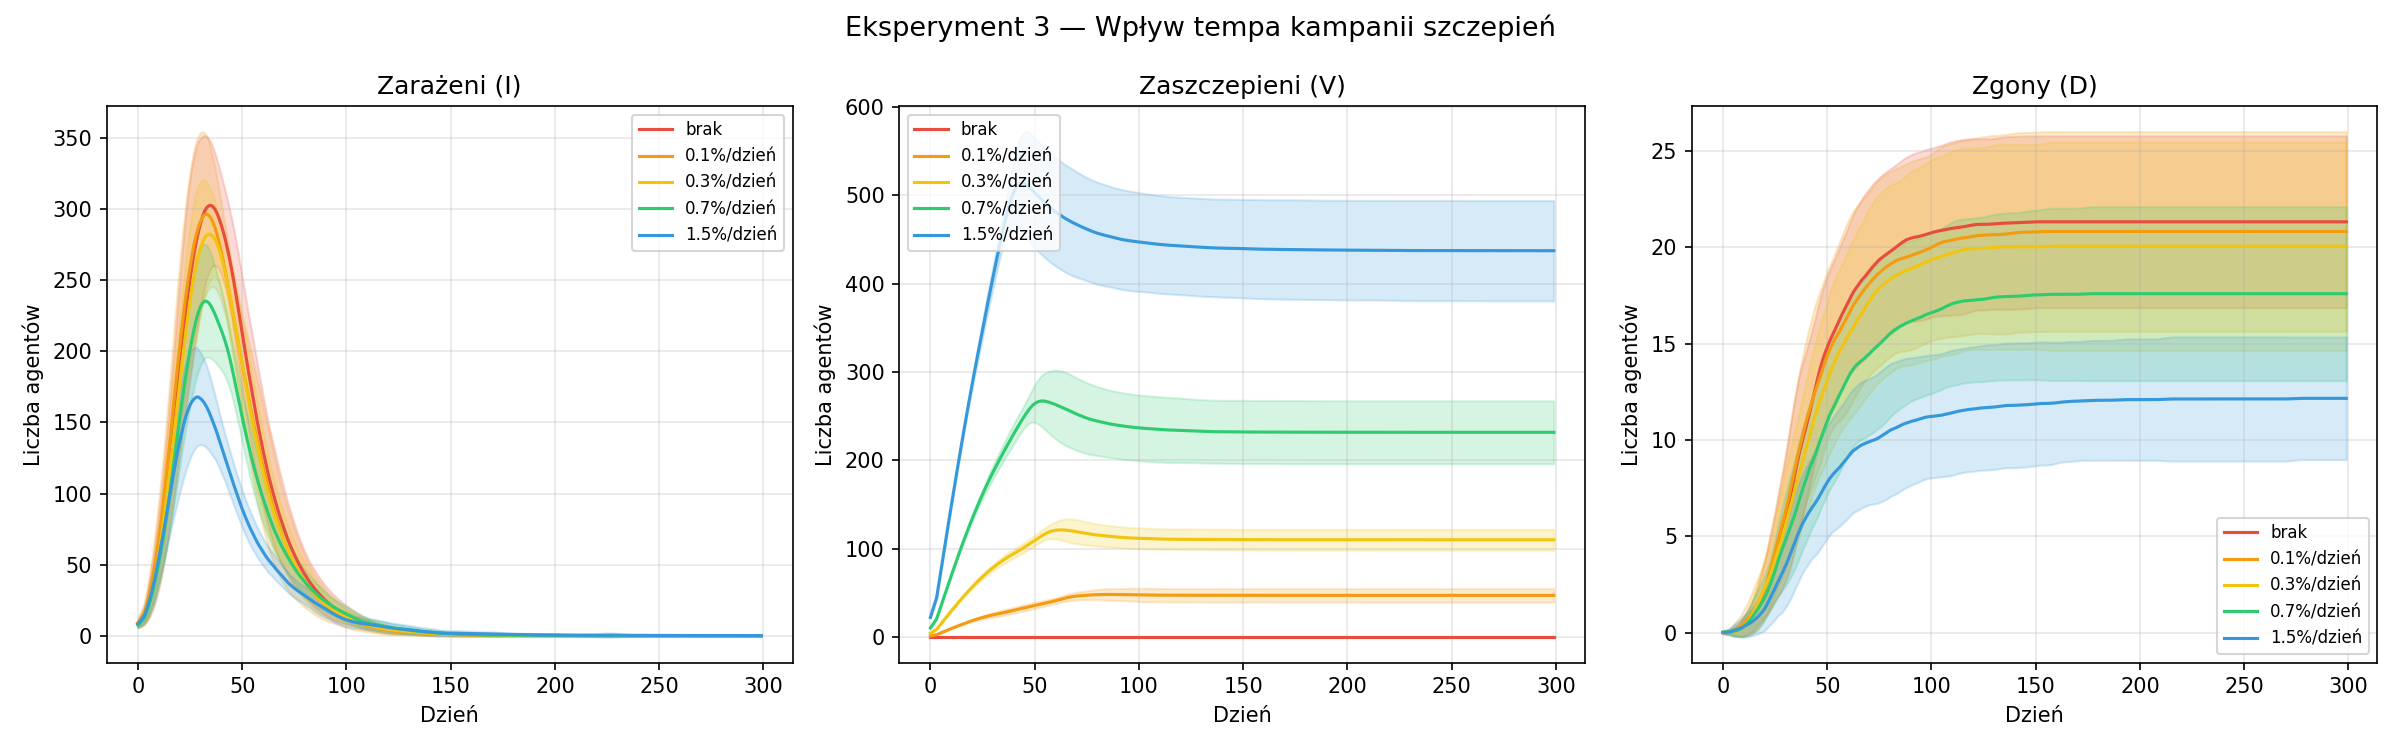
\includegraphics[width=\textwidth]{figures/exp3_vaccination.png}
  \caption{Wpływ tempa kampanii szczepień na przebieg epidemii.
  Wartość 0.3\%/dzień odpowiada średniemu tempu kampanii
  w Nowej Zelandii~\cite{baker2022newzealand}.
  Zacieniowane obszary reprezentują odchylenie standardowe z 30 uruchomień.}
  \label{fig:exp3}
\end{figure}

Pierwszy wykres pokazuje że szczepienia przy tempie poniżej
0.7\%/dzień mają ograniczony wpływ na szczyt zachorowań --
krzywe zarażonych dla wariantów 0.1\%, 0.3\% i braku szczepień
są zbliżone. Dopiero agresywna kampania 1.5\%/dzień wyraźnie
obniża szczyt i skraca czas trwania epidemii.

Drugi wykres potwierdza tę obserwację -- przy tempie 1.5\%/dzień
populacja jest szczepiona tak szybko, że znaczna jej część nabywa
odporność przed kontaktem z chorym. Dla pozostałych wariantów
liczba zaszczepionych stabilizuje się na niskim poziomie, bo
epidemia wygasa zanim kampania zdąży objąć większość populacji.

Trzeci wykres pokazuje że redukcja zgonów jest widoczna dopiero
przy tempie 0.7\%/dzień i wyższym. Przy tempie odpowiadającym
Nowej Zelandii (0.3\%/dzień) różnica względem braku szczepień
jest minimalna -- co sugeruje że sama kampania szczepień bez
wsparcia kwarantanną jest niewystarczająca przy przyjętych
parametrach bazowych.

\subsection{Eksperyment 4 -- Wpływ struktury wiekowej populacji}
\label{sec:exp4}

Eksperyment bada jak zmiana proporcji grup wiekowych wpływa na
śmiertelność i szczyt zachorowań. Trzy scenariusze odpowiadają
populacji młodej (70/20/10), przeciętnej (20/60/20) oraz
starzejącej się (10/50/40).

\begin{figure}[H]
  \centering
  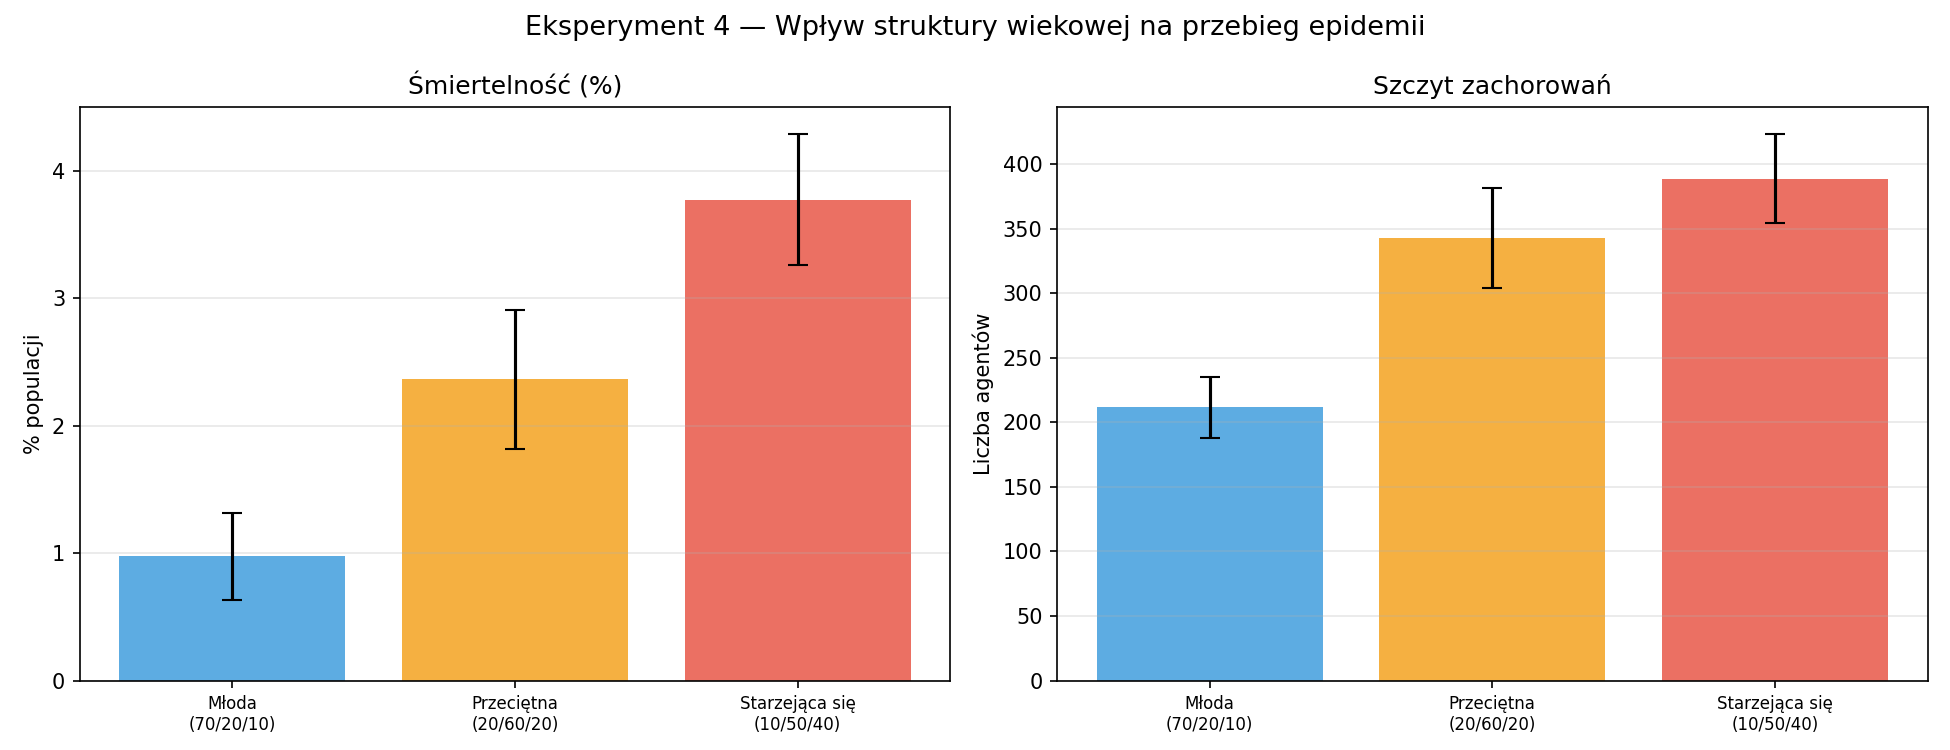
\includegraphics[width=.8\textwidth]{figures/exp4_age.png}
  \caption{Wpływ struktury wiekowej na śmiertelność i szczyt zachorowań.
  Słupki błędu reprezentują odchylenie standardowe z 30 uruchomień.}
  \label{fig:exp4}
\end{figure}

Pierwszy wykres pokazuje wyraźny wzrost śmiertelności wraz ze
starzeniem się populacji -- od około 1\% dla populacji młodej
do prawie 4\% dla starzejącej się. Wynik jest zgodny z danymi
epidemiologicznymi -- Levin et al.~\cite{levin2020age} wykazali
że śmiertelność COVID-19 rośnie wykładniczo z wiekiem.
Warto jednak zauważyć że odchylenie standardowe jest stosunkowo
duże, co wynika z losowości przydziału grup wiekowych w każdym
uruchomieniu.

Drugi wykres pokazuje że szczyt zachorowań również rośnie wraz
ze starzeniem się populacji, choć różnica między scenariuszem
przeciętnym a starzejącym się jest niewielka. Wynika to z faktu
że parametr $\beta$ jest jednakowy dla wszystkich grup wiekowych
-- wiek wpływa na śmiertelność i tempo zdrowienia, ale nie na
samą zaraźliwość agentów.

%%%%%%%%%%%%%%%%%%%%%%%%%%%%%%%%%%%%%%%%%%%%%%%%%%%%%%%%%%%%%%%%%%%%%%%%%%%%%%%
\section{\SectionTitleSummary}
\label{sec:conclusions}

Przeprowadzone eksperymenty pozwoliły na analizę wpływu kluczowych
parametrów epidemiologicznych na przebieg symulacji agentowej.

Współczynnik zaraźliwości $\beta$ ma istotny wpływ na dynamikę
epidemii -- wyższe wartości przyspieszają szczyt zachorowań
i skracają czas trwania epidemii. Zaobserwowano jednak tzw.
\textit{burnout effect}: przy bardzo wysokiej zaraźliwości
łączna śmiertelność może być niższa niż przy wartościach
umiarkowanych, ponieważ epidemia wygasa zanim zdąży objąć
całą podatną populację.

Strategie interwencyjne są wyraźnie skuteczne w ograniczaniu
liczby zachorowań i zgonów. Najefektywniejsza okazała się
kwarantanna oraz połączenie kwarantanny ze szczepieniami.
Należy jednak zaznaczyć ograniczenie modelu -- w rzeczywistości
idealna izolacja jest trudna do osiągnięcia ze względu na
kontakty domowe i nieprzestrzeganie zasad, co oznacza że
rzeczywista skuteczność kwarantanny byłaby niższa niż wynika
z symulacji.

Tempo kampanii szczepień ma mierzalny wpływ na przebieg epidemii,
jednak redukcja zgonów staje się wyraźna dopiero przy agresywnych
wariantach kampanii -- 0.7\% populacji dziennie i więcej. Tempo
odpowiadające danym z Nowej Zelandii (0.3\%/dzień) bez wsparcia
kwarantanną okazało się niewystarczające przy przyjętych parametrach
bazowych.

Struktura wiekowa populacji istotnie wpływa na śmiertelność --
w populacji starzejącej się jest ona niemal czterokrotnie wyższa
niż w młodej. Szczyt zachorowań jest natomiast stosunkowo podobny
dla populacji przeciętnej i starzejącej się, co wynika z faktu
że wiek nie wpływa na zaraźliwość agentów, a jedynie na tempo
zdrowienia i prawdopodobieństwo zgonu.

Dalsze badania mogłyby uwzględnić bardziej realistyczny model
kwarantanny z niepełną izolacją, wprowadzenie reinfection (powrotu
odpornych do puli podatnych) oraz kalibrację modelu do konkretnych
danych czasowych z wybranego kraju.
%%%%%%%%%%%%%%%%%%%%%%%%%%%%%%%%%%%%%%%%%%%%%%%%%%%%%%%%%%%%%%%%%%%%%%%%%%%%%%%
\printbibliography

%%%%%%%%%%%%%%%%%%%%%%%%%%%%%%%%%%%%%%%%%%%%%%%%%%%%%%%%%%%%%%%%%%%%%%%%%%%%%%%
\end{document}